\section{Methodology}

The robot that will be used is the adult-size humanoid robot Jaemi Hubo, see Fig.~\ref{fig:huboSch}.  Jaemi Hubo is a high gain position controlled device.  Each actuator is fead a reference position and is able to feed back the actuial position, the current through the actuator, and the actuator status (enabled or disabled).  Each actuator has an over current automatic disable rutine.  When this rutine is run the motor control is deactivated but feedback of the actuial position is still enabled.

\begin{figure}[thpb]
  \centering
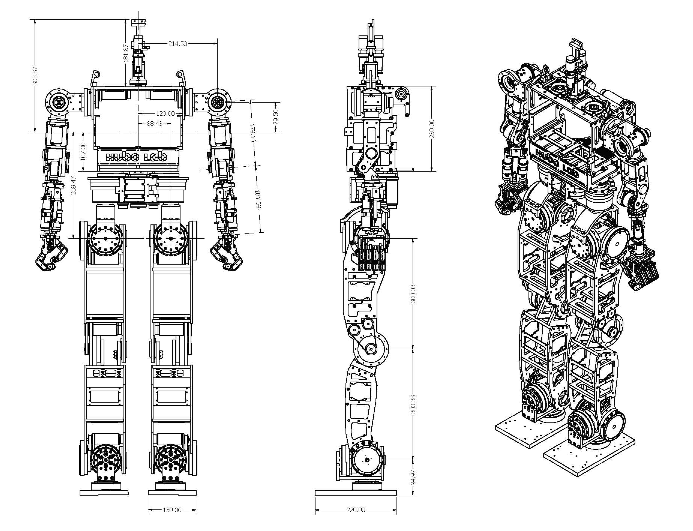
\includegraphics[width=1.0\columnwidth]{./pix/huboSch.png}
  \caption{Jaemi Hubo: 130cm tall 38kg (with battery) 40 degree of freedom, high gain position controlled adult-size humanoid robot }
  \label{fig:huboSch}
\end{figure}